\section{Примеры использования \LaTeX}
\paragraph{Параграф}
Какой-то текст, \textit{курсив} и \textbf{полужирный}.

\subsection{Отображение списков}
\subsubsection{Маркированный список}
Пример использования маркированного списка:

\begin{itemize}
  \item вариант 1
  \item вариант 2
  \item \dots
\end{itemize}

\subsubsection{Нумерованный список}
Пример использования нумерованного списка:

\begin{enumerate}
  \item шаг 1
  \item шаг 2
  \item ...
\end{enumerate}

\subsection{Пример вставки картинок}
\subsubsection{Пример вставки растровых картинок}
\begin{figure}[h]
  \center{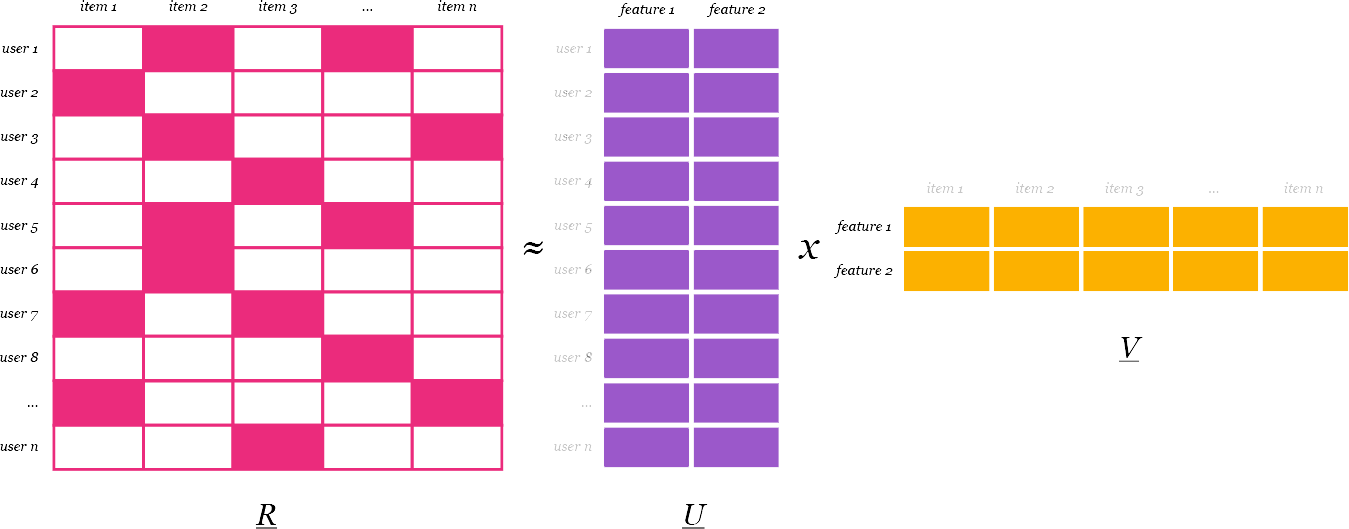
\includegraphics[width=\textwidth]{images/als-impliccit-collaborative-filtering-ruv.png}}
  \caption{Представление метода коллаборативной фильтрации}
  % \label{fig:image}
\end{figure}

\pagebreak
\subsubsection{Пример вставки векторных картинок}
\begin{figure}[h]
  \vspace{14pt}
  \begin{center}
    \begin{minipage}[h]{0.16\linewidth}
      \includesvg[width=0.9\textwidth]{images/Winding_Number_-2}
    \end{minipage}
    \begin{minipage}[h]{0.16\linewidth}
      \includesvg[width=0.9\textwidth]{images/Winding_Number_-1}
    \end{minipage}
    \begin{minipage}[h]{0.16\linewidth}
      \includesvg[width=0.9\textwidth]{images/Winding_Number_0}
    \end{minipage}
    \begin{minipage}[h]{0.16\linewidth}
      \includesvg[width=0.9\textwidth]{images/Winding_Number_1}
    \end{minipage}
    \begin{minipage}[h]{0.16\linewidth}
      \includesvg[width=0.9\textwidth]{images/Winding_Number_2}
    \end{minipage}
    \begin{minipage}[h]{0.16\linewidth}
      \includesvg[width=0.9\textwidth]{images/Winding_Number_3}
    \end{minipage}

    \vspace{14pt}
    \caption{Кривые с индексами от $-2$ (слева) до $3$ (справа).}
  \end{center}
\end{figure}

\subsection{Отображение таблиц}
Из CSV файла:
\begin{table}[h]
  \centering
  \caption{Матрица с предсказанными значениями}
  \csvautotabular{sheets/result.csv}
\end{table}

\subsection{Примеры вставки кода}
(пример вставки кода из файла можно посмотреть в приложениях 1 и 2)

пример вставки кода прямо сюда:
\par\medskip
\begin{lstlisting}
const confidence = matrix.scalar(alpha);
let X   = Matrix.random(users,   features);
let Y   = Matrix.random(stories, features);
let X_I = Matrix.identity(users);
let Y_I = Matrix.identity(stories);
let I   = Matrix.identity(features);
let lI  = I.scalar(lambda);
\end{lstlisting}

\subsection{Примеры использования формул}
$$S(u, i) = \frac{\sum\limits_{j \in N} W_{i,j} r_{u,i}}{\sum\limits_j |W_{i,j}|}$$

а также $R = U \times V$ и
\begin{equation}
  p_{ui} = \left\{\begin{array}{c}
    1, r_{ui} > 0 \\
    0, r_{ui} = 0 \\
  \end{array}\right.
\end{equation}

а также
\begin{multline*}
  \frac{1}{2\pi i} \int\limits_{S_\rho} \frac{f(z)}{z - z_0}\,dz - f(z_0) =\\
  = \frac{1}{2\pi i} \int\limits_{S_\rho} \frac{f(z)}{z - z_0}\,dz - \frac{1}{2\pi i} \int\limits_{S_\rho} \frac{f(z_0)}{z - z_0}\,dz =\\
  = \frac{1}{2\pi i} \int\limits_{S_\rho} \frac{f(z) - f(z_0)}{z - z_0}\,dz.
\end{multline*}

Пример формул с описанием значений:

У нас есть $Y-transpose-Y$ и $X-transpose-X$, независимые от $u$ и $i$, что означает, что мы можем вычислить его предварительно.
Итак, с учетом этого наши конечные уравнения имеют вид:
$$x_u = (Y^T Y + Y^T (C^u - I)Y + \lambda I)^{-1} Y^T C^u p(u)$$
$$y_i = (X^T X + X^T (C^i - I)X + \lambda I)^{-1} X^T C^i p(i)$$

\begin{ESKDexplanation}%[ширина]
  \item[где ] $X$ и $ Y$ - наши случайно инициализированные матрицы. Они будут попеременно обновляться.
  \item $Cu$ и $Ci$ - наши ценности доверия.
  \item $\lambda$ - регуляризатор для уменьшения переоснащения (мы используем 0.1).
  \item $p(u)$ и $p(i)$ - двоичное предпочтение. 1, если мы знаем предпочтение, и 0, если не знаем.
  \item $I$ матрица идентичности. Квадратная матрица с единицами по диагонали и нулями повсюду.
\end{ESKDexplanation}
